\documentclass[10pt,a4paper]{article}
\usepackage[utf8]{inputenc}
\usepackage[T1]{fontenc}
\usepackage[spanish,es-noshorthands]{babel}
\usepackage[margin=1.5cm, top=1.2cm, bottom=1.2cm]{geometry}
\usepackage{lmodern}
\usepackage{microtype}
\usepackage{graphicx}
\usepackage{booktabs}
\usepackage{tabularx}
\usepackage{enumitem}
\usepackage{titlesec}
\usepackage{xcolor}
\usepackage{hyperref}

\definecolor{acento}{HTML}{D9531E}
\definecolor{gris}{HTML}{555555}
\hypersetup{colorlinks=true, urlcolor=acento, linkcolor=acento}
\titleformat{\section}{\normalsize\bfseries\color{acento}}{}{0em}{}[\vspace{-0.9em}\textcolor{acento!40}{\rule{\linewidth}{0.4pt}}]
\titlespacing*{\section}{0pt}{0.6em}{0.1em}
\setlist{nosep, leftmargin=1.2em}
\setlength{\parindent}{0pt}
\setlength{\parskip}{0.3em}
\pagestyle{empty}

\begin{document}

{\LARGE\bfseries Trader cripto algorítmico: ¿le gana a comprar y mantener?}\\[0.3em]
{\color{gris}Tomás Moya Araya · Ingeniero Civil Industrial · Proyecto personal de análisis de datos · Septiembre 2026}\\[-0.4em]
\textcolor{acento}{\rule{\linewidth}{1.2pt}}

\section{Pregunta y enfoque}
¿Un sistema de reglas que busca oportunidades, planifica cada operación y controla el riesgo rinde más que comprar y
esperar? Construí el sistema en Python (15 criptomonedas, velas de 4 horas, datos de Binance) y lo evalué con un
\textbf{backtest vela a vela sobre 6 años de datos reales (2020--2026)}, con capital ficticio.

\section{Método}
\begin{itemize}
  \item \textbf{Pipeline:} extracción por API con caché incremental $\rightarrow$ indicadores (EMA, RSI, ATR, volumen)
        $\rightarrow$ 5 setups como reglas explícitas $\rightarrow$ plan (entrada, stop, objetivo) $\rightarrow$
        motor de riesgo con 8 controles y veto $\rightarrow$ cartera simulada con límites de exposición.
  \item \textbf{Realismo:} sin información futura en ninguna vela; entrada en la apertura siguiente; comisiones y
        deslizamiento; ante ambigüedad intra-vela se asume el peor caso.
  \item \textbf{Validación:} tramos de entrenamiento (2023--24) y validación (2025--26), y luego una prueba sobre
        \textbf{2020--23, datos nunca vistos}. Cada mejora se evaluó con un criterio de adopción fijado de antemano.
\end{itemize}

\section{Resultados}
\begin{minipage}[t]{0.47\linewidth}
\vspace{0pt}
\small
\begin{tabularx}{\linewidth}{@{}Xrr@{}}
\toprule
 & \textbf{2020--23} & \textbf{2023--26} \\
\midrule
Operaciones            & 250     & 300 \\
Tasa de acierto        & 48,8\%  & 47,3\% \\
Expectativa por operación & +0,27R & +0,20R \\
Retorno del sistema    & +86\%   & +63\% \\
Caída máxima sistema   & $-$13\% & $-$14\% \\
\midrule
Retorno BTC (mantener) & +153\%  & +210\% \\
Caída máxima BTC       & $-$77\% & $-$53\% \\
\bottomrule
\end{tabularx}\\[0.3em]
{\footnotesize\color{gris}R = monto arriesgado por operación (1\% del capital).}

\vspace{0.5em}
\textbf{36 inicios posibles, plazo de 3 años (\$1.000):}\\[0.2em]
\begin{tabularx}{\linewidth}{@{}Xrr@{}}
\toprule
 & \textbf{Sistema} & \textbf{BTC} \\
\midrule
Retorno típico (mediana)      & +45\%   & \textbf{+129\%} \\
Peor resultado                & \textbf{+22\%} & +4\% \\
Punto más bajo de los \$1.000 & \textbf{\$931} & \$262 \\
Veces que gana                & 9       & \textbf{27} \\
\bottomrule
\end{tabularx}
\end{minipage}\hfill
\begin{minipage}[t]{0.5\linewidth}
\vspace{0pt}
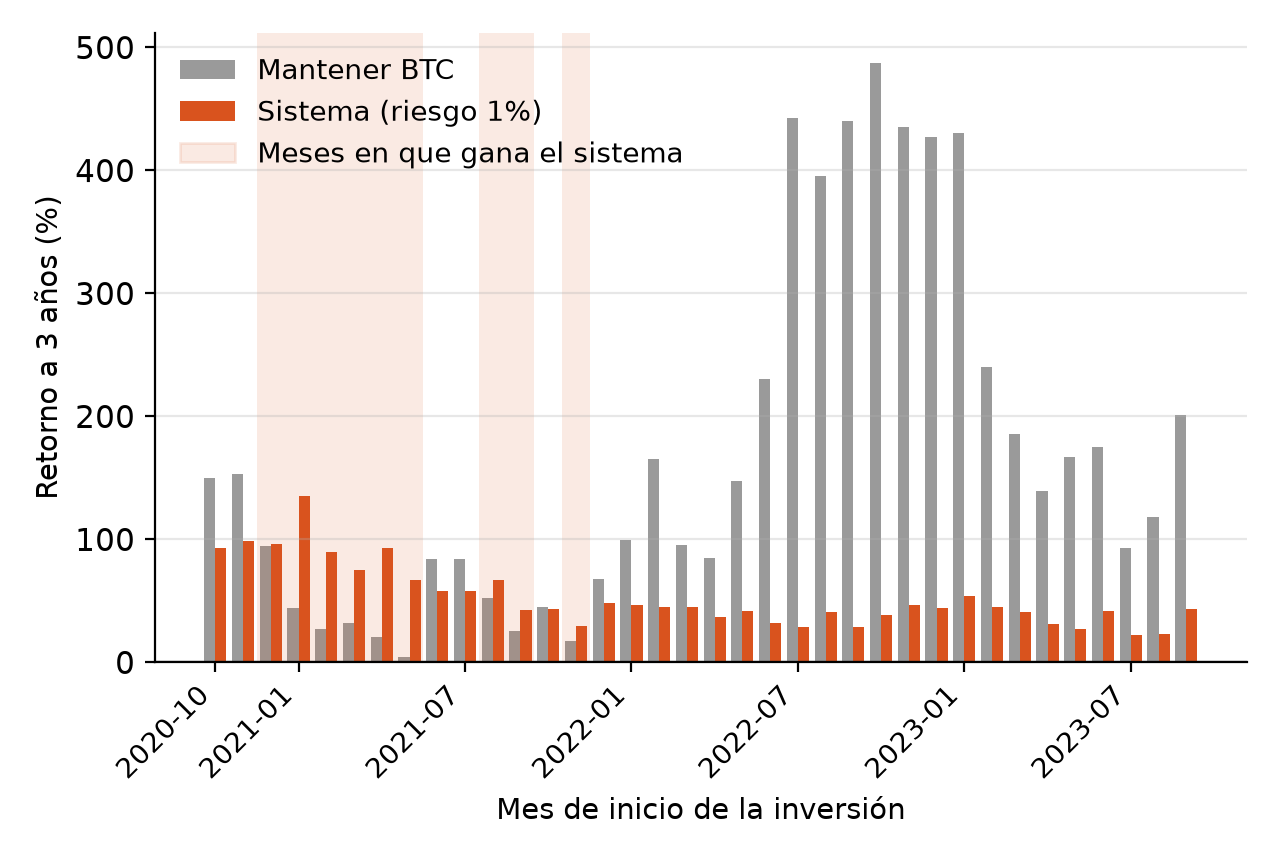
\includegraphics[width=\linewidth]{img/informe_ventanas.png}\\
{\footnotesize\color{gris}Retorno a 3 años si se invierte \$1.000 en cada mes de inicio. El sistema solo gana
cuando se parte cerca del máximo de 2021.}
\end{minipage}

\section{Qué se probó y qué se descartó}
\small
\begin{tabularx}{\linewidth}{@{}lXl@{}}
\toprule
\textbf{Cambio} & \textbf{Evidencia} & \textbf{Decisión} \\
\midrule
Eliminar 2 setups (Pullback, Continuación) & Perdían en ambos tramos ($-$0,12R y $-$0,17R) & Adoptado \\
Operar solo en tendencia alcista & +0,16R $\rightarrow$ +0,27R en datos nunca vistos & Adoptado \\
Stop dinámico & Más ganancia por operación, pero menos operaciones y más caída en 2023--26 & Descartado \\
Fuerza relativa vs BTC & Mejora un periodo y empeora el otro & Descartado \\
Subir el riesgo a 2--3\% & Con 3\% rinde \emph{menos} que con 1\% en 2023--26 & No adoptado \\
\bottomrule
\end{tabularx}
\normalsize

\textbf{Error propio corregido:} el filtro de tendencia lo elegí mirando toda la historia, lo que contaminaba la
validación. Lo detecté y lo sometí a una prueba limpia sobre 2020--23 antes de adoptarlo.

\section{Conclusiones}
\begin{itemize}
  \item El sistema tiene una \textbf{ventaja real pero delgada} (+0,20R a +0,27R), estable en mercados muy distintos,
        y en su peor momento \textbf{cae entre 4 y 6 veces menos} que BTC.
  \item \textbf{En retorno no le gana a mantener BTC} en 3 de cada 4 escenarios: invierte en promedio solo $\sim$15\% del
        capital y 2020--26 fue un periodo excepcional para BTC. Su valor está en el control del riesgo.
  \item \textbf{Un backtest riguroso sirve sobre todo para descartar:} de 8 variantes probadas, solo 2 se adoptaron.
  \item \textbf{Limitaciones:} solo compras; sesgo de supervivencia (monedas actuales, no las que colapsaron). El paper
        trading en tiempo real comenzó en septiembre de 2026.
\end{itemize}

\vfill
{\footnotesize\color{gris}\textbf{Stack:} Python, pandas, ccxt, matplotlib, openpyxl, YAML, Programador de tareas de Windows.\\
\textbf{Código y metodología:} \href{https://github.com/tomasmoyaaraya/trader-cripto-backtest}{github.com/tomasmoyaaraya/trader-cripto-backtest}
· Proyecto de análisis con capital ficticio; no es asesoría financiera.}

\end{document}
